\documentclass{beamer}

\mode<presentation> {
  \usetheme{Dresden}
  \usecolortheme{orchid}

  %\setbeamertemplate{footline} % To remove the footer line in all slides uncomment this line
  \setbeamertemplate{footline}[page number] % To replace the footer line in all slides with a simple slide count uncomment this line

  \setbeamertemplate{navigation symbols}{} % To remove the navigation symbols from the bottom of all slides uncomment this line
}

\usepackage{graphicx}
\usepackage{booktabs}
\usepackage[german]{babel}
\usepackage[utf8]{inputenc}

\title[Tests]{Tests}

\author{Schwarz, Christian (s68419)}
%\institute[HTW-DD]{Hochschule für Technik und Wirtschaft, Dresden}

\date{\today}

\begin{document}

\begin{frame}
  \titlepage
\end{frame}

\begin{frame}
  \frametitle{Überblick}
  \tableofcontents
\end{frame}

\section{Aufgabenbereich}

\begin{frame}
  \frametitle{Aufgabenbereich}
  \begin{itemize}
  \item Testen der aktuellen Version
  \item Prüfung auf Sicherheit
  \end{itemize}
\end{frame}

\section{Entstehung eines Testberichtes}
\begin{frame}
  \frametitle{Entstehung eines Testberichtes}
  \begin{itemize}
  \item Testfälle durchgehen und Ergebnis festhalten
  \item Testdokumentation erzeugen
    \begin{itemize}
    \item Testberichte nach LaTeX übersetzen
    \item (Testberichte parsen)
    \item (Diagramm erzeugen)
    \item Testdokumentation zusammensetzen
    \item PDF erzeugen
    \end{itemize}
  \end{itemize}
\end{frame}

\begin{frame}
  \frametitle{Testbericht in Rohform}
  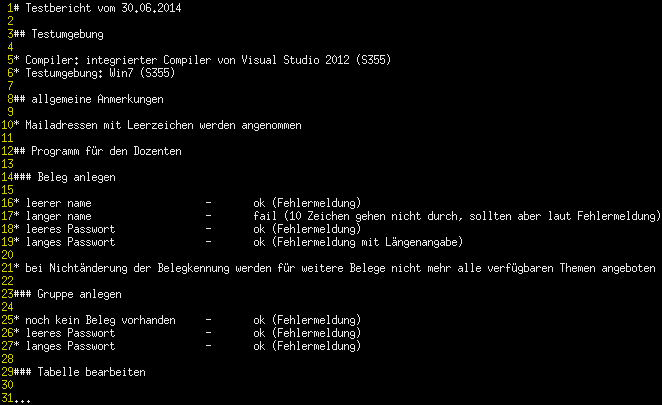
\includegraphics[width=\textwidth]{bericht.png}
\end{frame}

\begin{frame}
  \frametitle{Zwischenprodukt}
  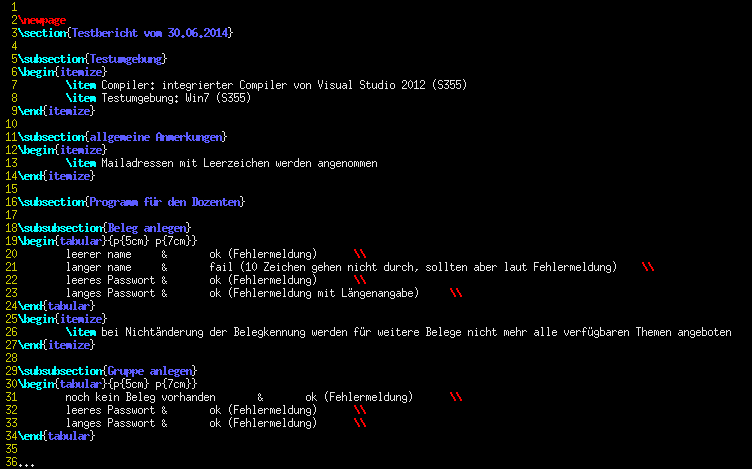
\includegraphics[width=\textwidth]{latex.png}
\end{frame}

\begin{frame}
  \frametitle{Endprodukt}
  \begin{center}
  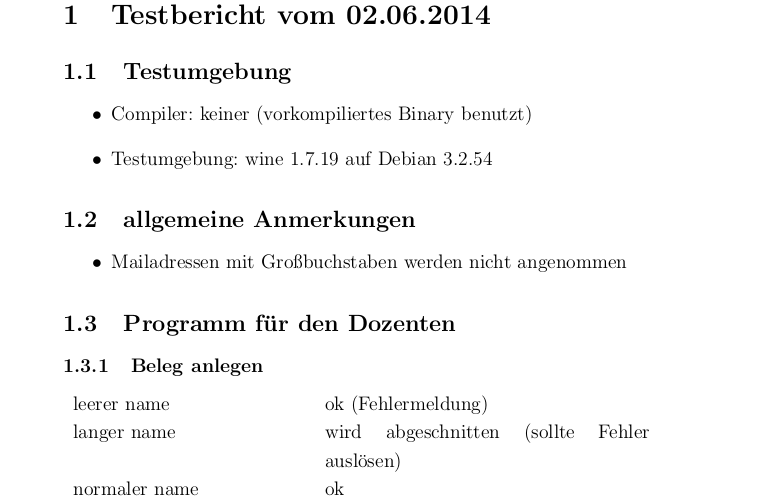
\includegraphics[width=0.7\textwidth]{pdf.png}
  \end{center}
\end{frame}

\section{Statistik}
\begin{frame}
  \frametitle{Zahlen}
  \begin{tabular}{l l}
    durchgeführte Tests: & 5 \\
    durchschnittliche Anzahl Testfälle: & 39 \\
    durchschnittliche Fehlerrate: & 32.26\% \\
  \end{tabular}
\end{frame}

\begin{frame}
  \frametitle{Diagramm}
  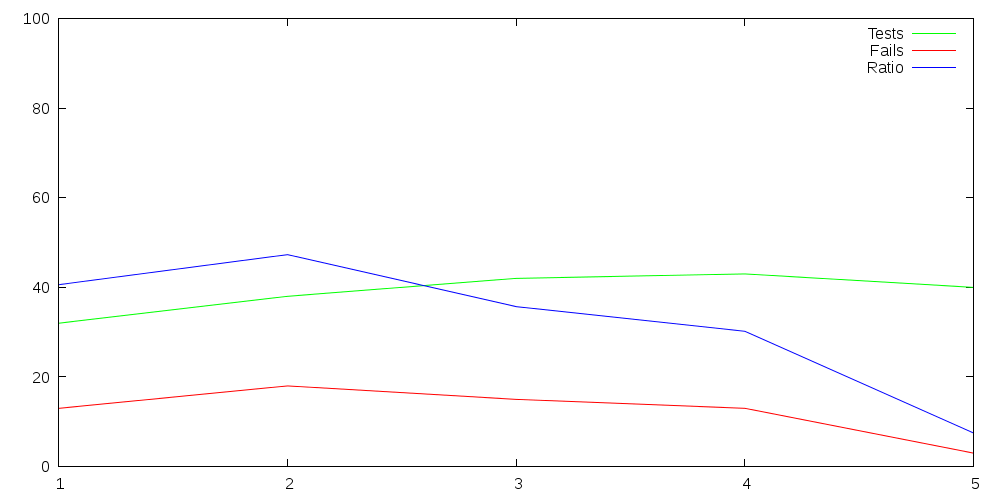
\includegraphics[width=\textwidth]{dia.png}  
\end{frame}

\section{Reflexion}
\begin{frame}
  \frametitle{Was habe ich gelernt?}
  \begin{itemize}
    \item Ruby-Kenntnisse verbessert
    \item .NET und wine zum laufen gebracht
    \item Techniken zum umformatieren von Text erlernt
    \item \LaTeX-Kenntnisse vertieft
  \end{itemize}
\end{frame}

\begin{frame}
  \frametitle{Was hat sich bewährt, was nicht?}

  hat sich bewährt:
  \begin{itemize}
  \item Ruby-Script zur automatischen Generierung der Dokumentation
  \item Verwendung von \LaTeX zur Dokumentation der Tests
  \item Nutzung von GNUplot zur Erzeugung von Diagrammen
  \end{itemize}
  \vspace{0.5cm}

  hat sich nicht bewährt:
  \begin{itemize}
  \item Nutzung von wine zum Testen von .NET-Anwendungen
  \end{itemize}
\end{frame}

\begin{frame}
  \frametitle{Was würde ich wieder so machen, was nicht?}

  würde ich wieder so machen:
  \begin{itemize}
  \item Verwendung von \LaTeX \, zur Dokumentation der Tests
  \item Nutzung von GNUplot zur Erzeugung von Diagrammen
  \end{itemize}
  \vspace{0.5cm}

  würde ich anders machen:
  \begin{itemize}
  \item Testingframework nutzen
  \item Implementation mit Unit-Tests begleiten
  \end{itemize}
\end{frame}

\section{Sicherheitshinweise}
\begin{frame}
  \frametitle{Sicherheitshinweise}
  \begin{itemize}
    \item Zugangsdaten werden im Klartext übertragen
    \item keine Nutzerverwaltung innerhalb der Datenbank
  \end{itemize}
\end{frame}

\end{document}
